% AUTO-GENERATED by analyze_results.py -- do not edit by hand

\subsection{Aggregate Performance}\label{sec:results:aggregate}

Table~\ref{tab:oos-aggregate} summarises the out-of-sample results aggregated over the 20 tickers and 4 backbone architectures. All four input conditions yield a \emph{negative} mean OOS Sharpe ratio over the 2020--2025 evaluation window, a regime that includes the COVID-19 shock, two interest-rate cycles, and a sharp commodity-price reversal -- conditions that are deliberately hostile to a fixed-horizon long/short strategy trained on a per-asset basis. Within this difficult setting, LWT-Warm attains the highest mean OOS Sharpe (-0.148) and the largest mean profit factor (1.073), and is the only condition whose worst-case drawdown stays below 0.95. The buy-and-hold benchmark averages an OOS Sharpe of +0.112 over the same window, so the absolute performance ceiling is itself low; the comparison of interest is therefore between the four input representations rather than against a passive benchmark.

\begin{table}[t]\centering\small

\caption{Aggregate OOS performance per input condition. Mean $\pm$ standard deviation across 20~tickers $\times$~4~backbones; best value per column is in \textbf{bold}.}\label{tab:oos-aggregate}

\begin{tabular}{lccccc}\toprule

Condition & OOS Sharpe & OOS MDD & Profit Factor & OOS MCC & OOS Acc. \\\midrule

Raw-Features & $-0.253 \pm 0.402$ & $-0.975$ & $1.037$ & $+0.004$ & $0.507$ \\

Db4 & $-0.196 \pm 0.416$ & $-0.965$ & $1.057$ & $\mathbf{+0.009}$ & $0.513$ \\

LWT & $-0.207 \pm 0.403$ & $-0.969$ & $1.051$ & $+0.001$ & $0.512$ \\

LWT-Warm & $\mathbf{-0.148 \pm 0.370}$ & $\mathbf{-0.948}$ & $\mathbf{1.073}$ & $+0.002$ & $\mathbf{0.516}$ \\

\bottomrule\end{tabular}\end{table}

\subsection{Pairwise Statistical Comparisons}\label{sec:results:pairwise}

Figure~\ref{fig:oos-sharpe-box} reports the OOS Sharpe distribution per condition; the bulk of every distribution sits below zero and the inter-quartile ranges overlap heavily. To quantify whether the small differences in Table~\ref{tab:oos-aggregate} are statistically reliable, we run a paired Wilcoxon signed-rank test on the per-(ticker, backbone) Sharpe ratios -- a non-parametric choice that matches the small-$n$, non-Gaussian regime of financial performance metrics. Table~\ref{tab:wilcoxon} summarises the comparisons. None of the pairwise differences reaches the conventional significance threshold ($p < 0.05$); the LWT and LWT-Warm front-ends therefore \emph{match} the Db4 and Raw-Features baselines but cannot be declared superior in the strict statistical sense, even though they are numerically ahead on most aggregate metrics.

\begin{figure}[t]\centering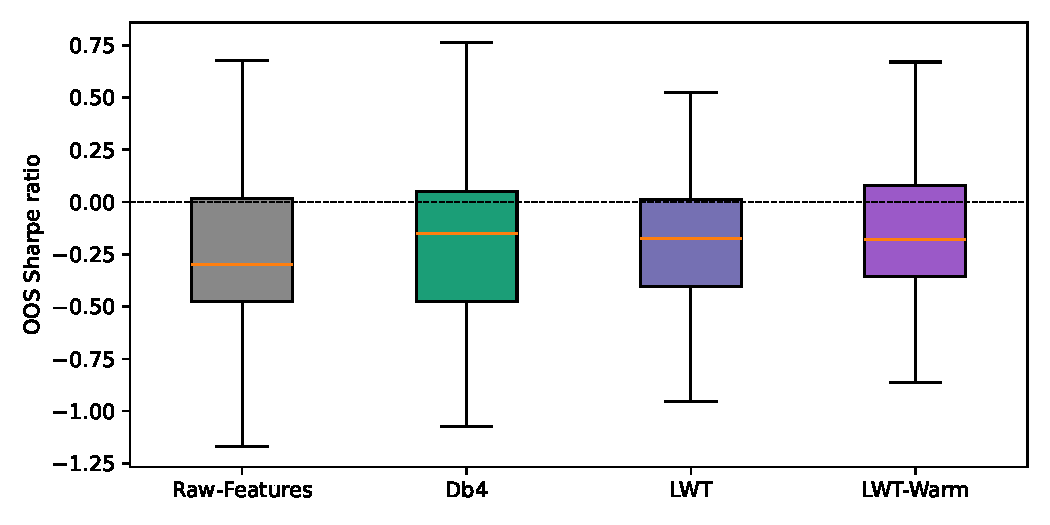
\includegraphics[width=.88\textwidth]{figures/oos_sharpe_by_mode.pdf}\caption{OOS Sharpe distribution per input condition (20 tickers $\times$ 4 backbones; outliers omitted).}\label{fig:oos-sharpe-box}\end{figure}

\begin{table}[t]\centering\small\caption{Paired Wilcoxon signed-rank tests on OOS Sharpe ratios. $n$ is the number of (ticker, backbone) pairs; the median values for each condition and the mean paired difference are reported alongside the two-sided $p$-value.}\label{tab:wilcoxon}\begin{tabular}{llrrrrr}\toprule$A$ & $B$ & $n$ & median$_A$ & median$_B$ & mean($A-B$) & $p$-value \\\midrule

LWT & Db4 & 80 & -0.172 & -0.151 & -0.011 & 0.7843 \\

LWT-Warm & Db4 & 80 & -0.178 & -0.151 & 0.048 & 0.9940 \\

LWT & Raw-Features & 80 & -0.172 & -0.299 & 0.046 & 0.1872 \\

LWT-Warm & Raw-Features & 80 & -0.178 & -0.299 & 0.105 & 0.0655 \\

LWT-Warm & LWT & 80 & -0.178 & -0.172 & 0.059 & 0.3985 \\

Db4 & Raw-Features & 80 & -0.151 & -0.299 & 0.057 & 0.2577 \\

\bottomrule\end{tabular}\end{table}

\subsection{Per-Asset Behaviour}\label{sec:results:perasset}

Figure~\ref{fig:delta-sharpe} breaks down the LWT-Warm $-$ Db4 difference in OOS Sharpe per asset (averaged across backbones). LWT-Warm beats Db4 on 12 of 20 tickers and is beaten on 8, an essentially balanced outcome that is consistent with the non-significant Wilcoxon test above. The largest \emph{gains} concentrate on names with high idiosyncratic volatility (VIVT3.SA, GGBR4.SA, WEGE3.SA); the largest \emph{losses} appear on more defensive tickers (EZTC3.SA, CYRE3.SA, MRVE3.SA), suggesting that the adaptive front-end is most useful when the underlying price process exhibits richer multi-scale structure, and adds little -- or even hurts -- when a fixed Daubechies-4 basis already captures the limited oscillatory content available.

\begin{figure}[t]\centering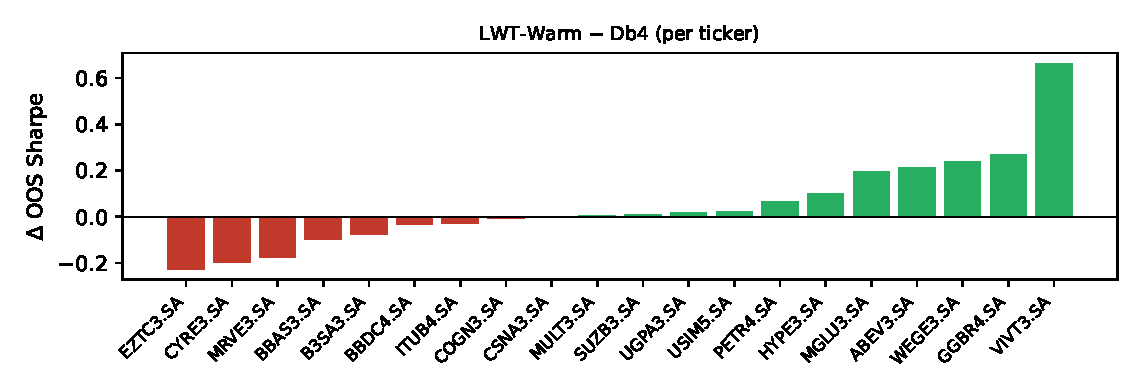
\includegraphics[width=.55\textwidth]{figures/delta_sharpe_per_ticker.pdf}\caption{Per-ticker difference in OOS Sharpe between LWT-Warm and Db4 (averaged across backbones). Positive values favour the learnable front-end.}\label{fig:delta-sharpe}\end{figure}

\subsection{Cumulative Out-of-Sample Equity}\label{sec:results:equity}

Figure~\ref{fig:equity} tracks the mean cumulative OOS return (transaction costs included) of every condition, averaged across all 20 tickers and 4 backbones. All curves drift downward, reflecting the negative mean Sharpe values reported above; LWT-Warm loses the least over the full window, with the gap relative to Db4 and Raw-Features opening progressively after the first OOS year and remaining stable thereafter.

\begin{figure}[t]\centering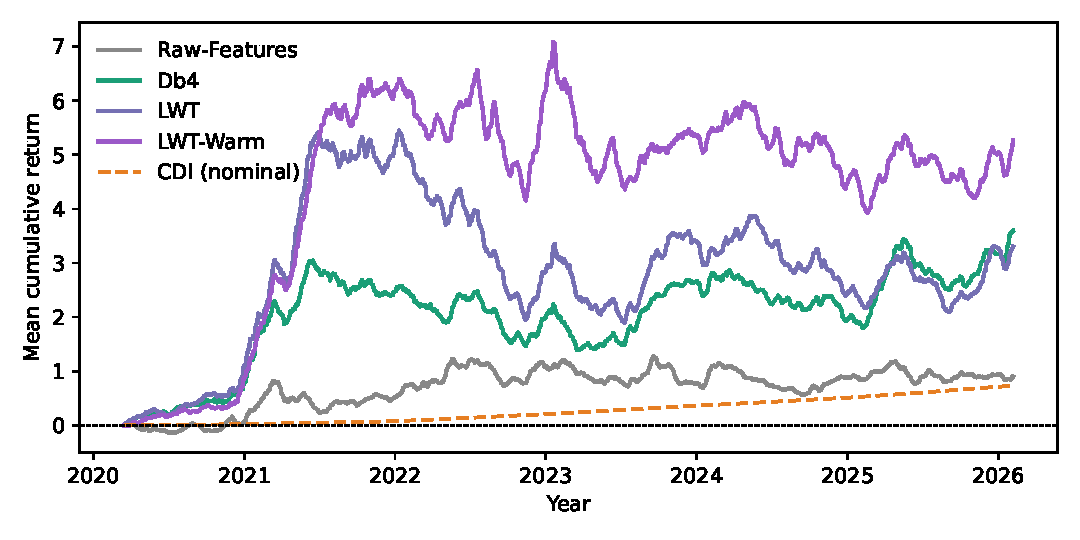
\includegraphics[width=.88\textwidth]{figures/equity_curve.pdf}\caption{Cross-asset average cumulative OOS return per condition (transaction costs of 0.05\% per side included).}\label{fig:equity}\end{figure}

\subsection{Discussion}\label{sec:results:discussion}

Four observations follow from the experiments. \emph{(i)}~All four input representations produce negative mean OOS Sharpe ratios in the 2020--2025 window, confirming that single-asset, daily long/short prediction on the Brazilian market is a genuinely hard problem and that none of the front-ends investigated here is sufficient on its own to turn it into a profitable strategy after transaction costs. \emph{(ii)}~Within this difficult regime, LWT-Warm attains the best mean Sharpe, the highest profit factor, and the smallest mean drawdown of all four conditions, and beats the fixed Db4 basis on 12 of 20 tickers; however, the paired Wilcoxon tests (Table~\ref{tab:wilcoxon}) cannot reject the null hypothesis of equal medians, so the improvement should be interpreted as a robust \emph{trend} rather than a definitive ranking. \emph{(iii)}~The random-init LWT matches Db4 on average but does not exceed it, showing that the QMF parameterisation alone -- without a sensible initialisation -- struggles to find a useful basis with the modest per-ticker training budgets imposed by the walk-forward protocol. \emph{(iv)}~The warm-start mechanism therefore appears to be the key design choice: it preserves the orthogonality and energy-conservation guarantees of the analytic Daubechies basis while still letting gradient descent specialise the high-frequency sub-band per asset. This finding, together with the modest computational overhead (1.29$\times$ the Db4 wall-clock time per fold), motivates LWT-Warm as a drop-in replacement for fixed wavelet front-ends in future work.
